\subsection{Präsentationsaufbau}\label{hw_testaufbau}
\begin{figure}[H]
    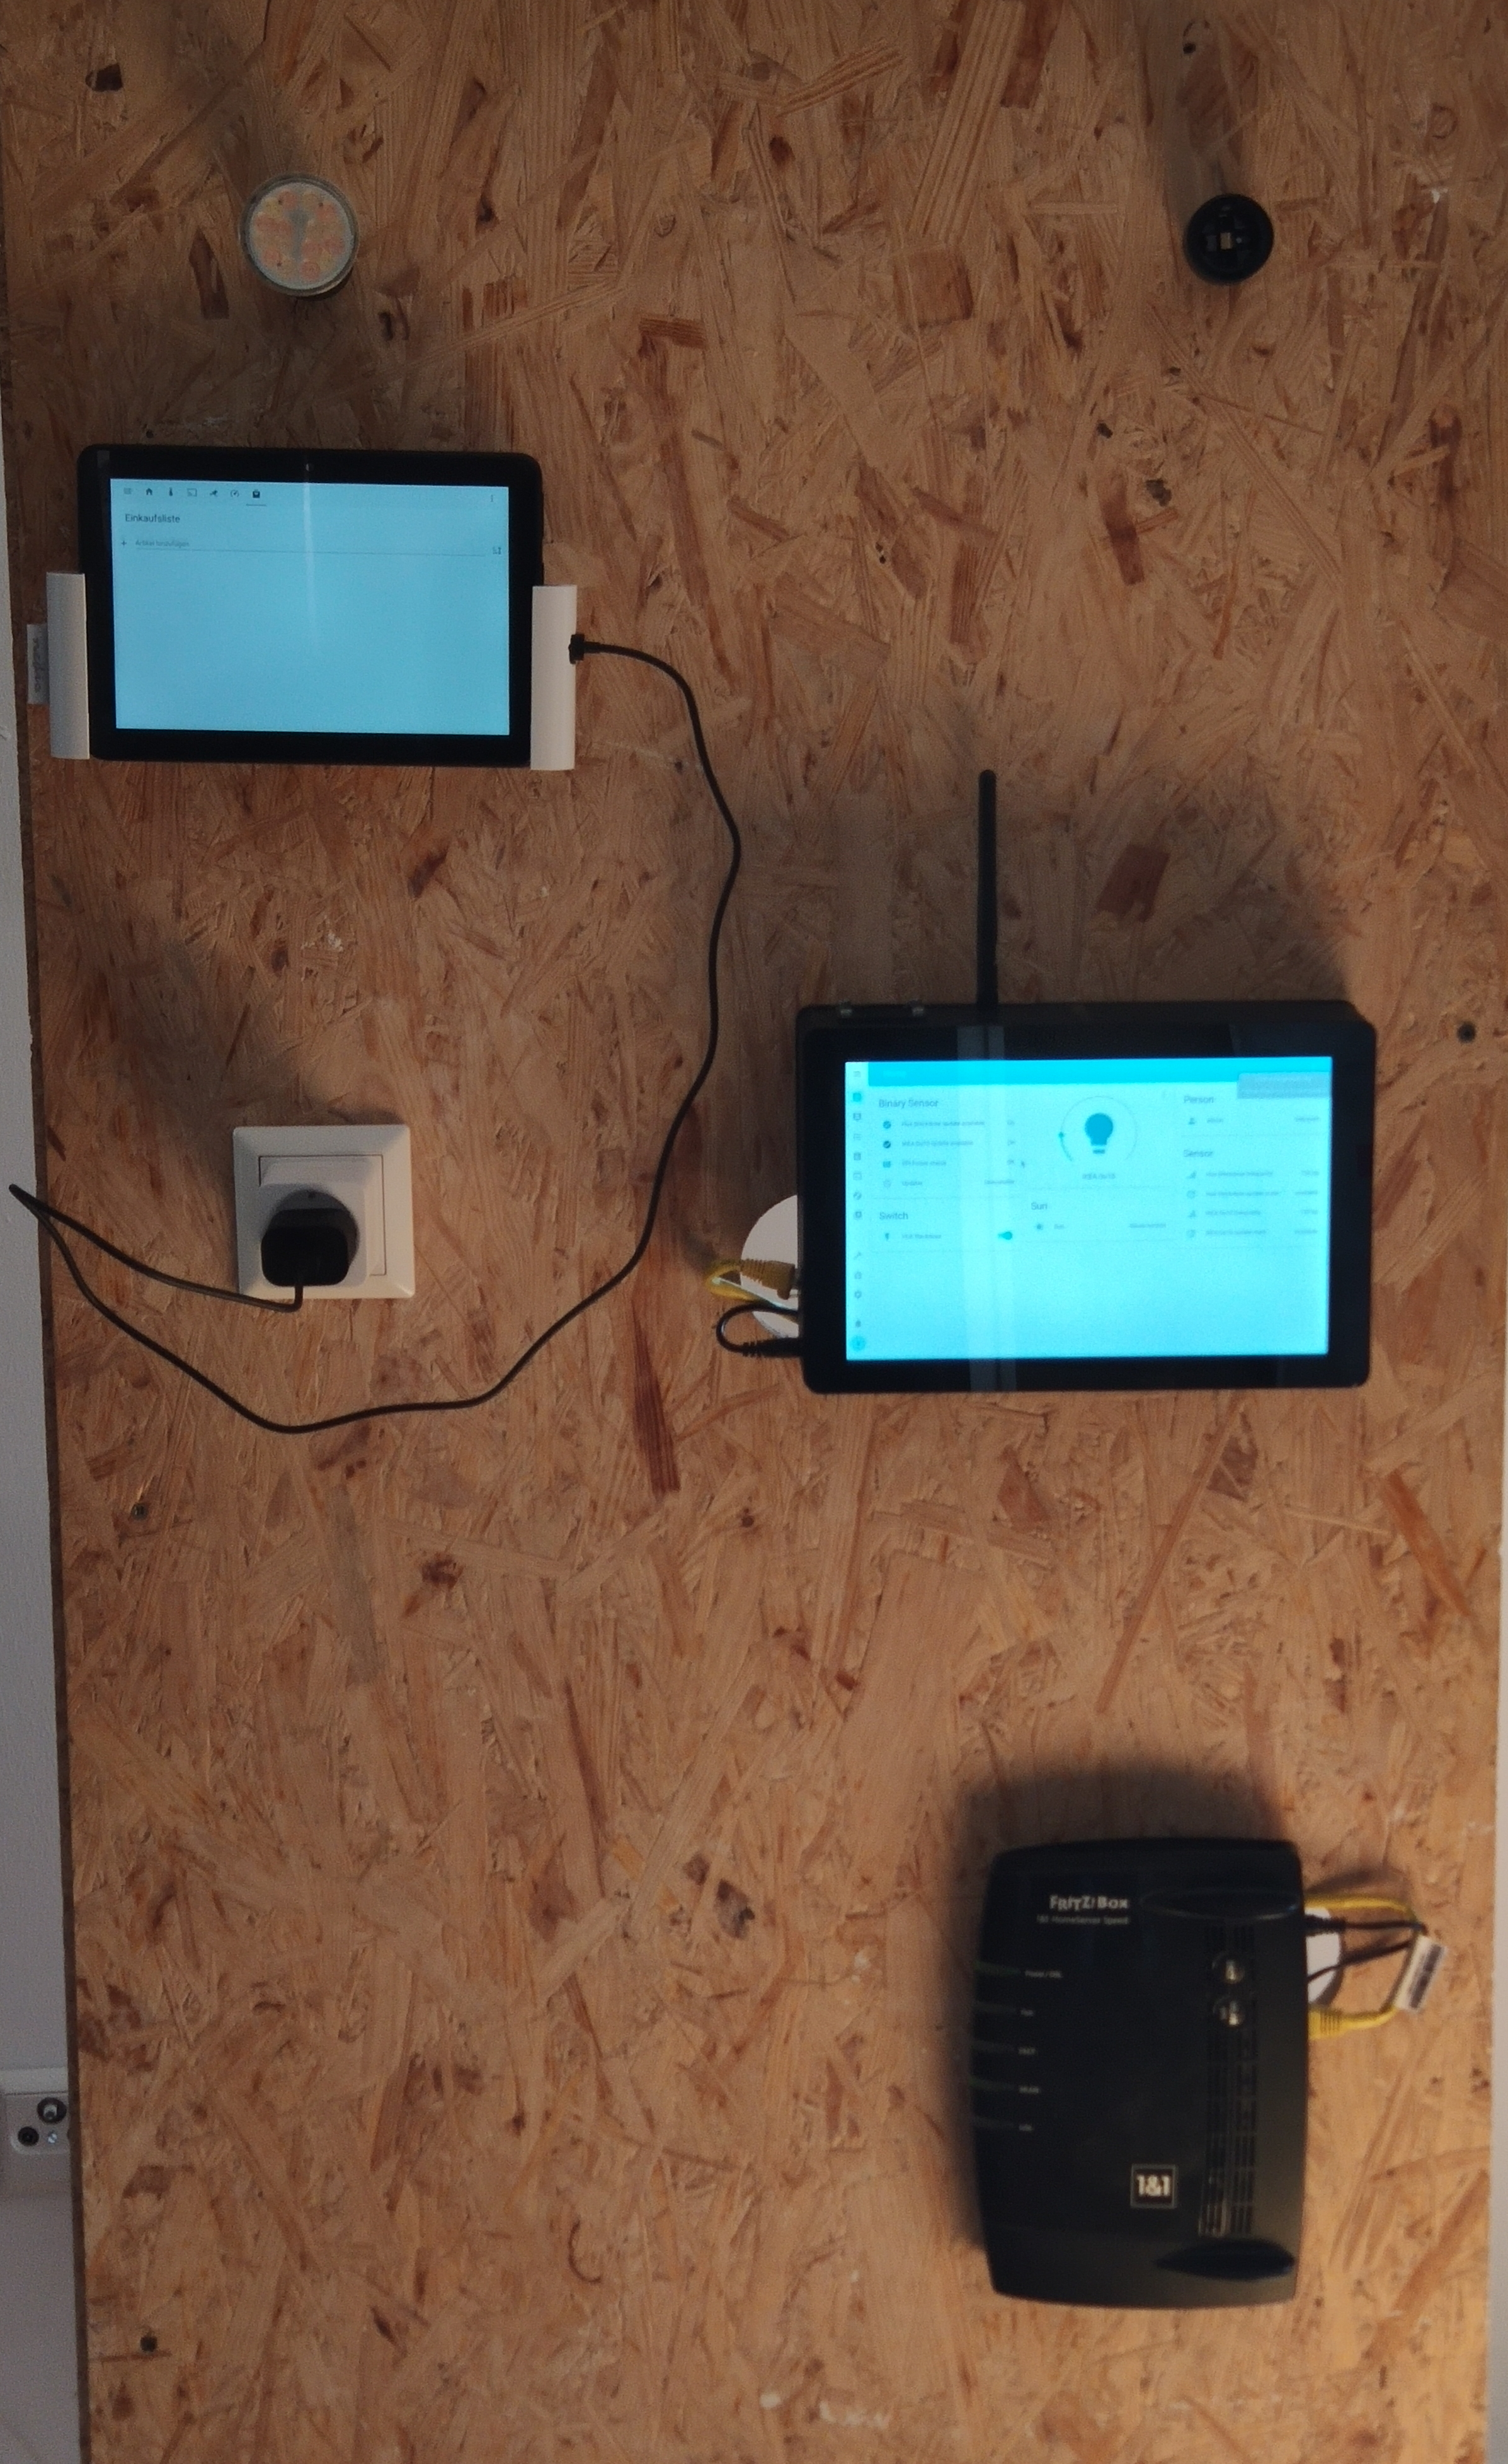
\includegraphics[width=0.5\textwidth]{img/t1.jpg}
    \caption[Präsentationsaufbau]{Präsentationsaufbau}
    \label{fig:praesentationsaufbau}
\end{figure}
Um die Ergebnisse unseres Technikerarbeit und unserem Prototypen präsentieren zu können, haben wir einen Präsentationsaufbau auf Basis einer OSB-3-Verlegeplatte gebaut (vgl. Abb. \ref{fig:praesentationsaufbau}: \nameref{fig:praesentationsaufbau}).
Dieser ist neben der Smart Home Zentrale mit einem Router, zwei Zigbee-fähigen Glühbirnen, einer Phillips Hue Zigbee Steckdose und einem Amazon Fire8 HD Tablet ausgestattet.
Der Aufbau soll die Funktion der Smart Home Zentrale in der Steuerung von Smart Home Komponenten praktisch aufzeigen und wurde von uns selbst gebaut.
